\input sys/inputs.tex
\usepackage{pgf,tikz}

\begin{document}

\bigheading{Secret Service}

% \info{task_name}{infile}{outfile}{points}{timelimit}{memlimit}
% leave this values, if you are not interested
\info{secret}{stdin}{stdout}{100}{2000 ms}{1 GB}

The secret service managed to obtain a plan of an enemy military object. The
plan of the object is a square-shaped black-and-white image. The following
compression algorithm was used for its transmission:

\begin{itemize}[nolistsep]

\item A square covered with only one color is encoded as one letter --
  \texttt{B} in the case of the black color, or \texttt{W} in the case of the
  white color.

\item A square which is not entirely covered with only one color is divided into
  four squares of the same size. Each of them is recursively encoded using the
  same algorithm. The original square is then encoded as a string wrapped in
  parentheses in which the inner squares are encoded in sequence -- the upper
  left square, the upper right square, the lower left square and the lower right
  square.

\end{itemize}

For example, an image encoded as \texttt{(B(WWBW)(WBWW)(WWWB))} looks like this:

\begin{center}
  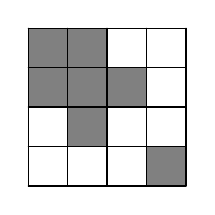
\begin{tikzpicture}[line cap=round,line join=round,x=0.5cm,y=0.5cm]
    \fill[fill=gray] (0,2) -- (1,2) -- (1,3) -- (0,3) -- cycle;
    \fill[fill=gray] (0,3) -- (1,3) -- (1,4) -- (0,4) -- cycle;
    \fill[fill=gray] (1,1) -- (2,1) -- (2,2) -- (1,2) -- cycle;
    \fill[fill=gray] (1,2) -- (2,2) -- (2,3) -- (1,3) -- cycle;
    \fill[fill=gray] (1,3) -- (2,3) -- (2,4) -- (1,4) -- cycle;
    \fill[fill=gray] (2,2) -- (3,2) -- (3,3) -- (2,3) -- cycle;
    \fill[fill=gray] (3,0) -- (4,0) -- (4,1) -- (3,1) -- cycle;

    \foreach \x in {0,...,4}
      \draw [line width=0.5pt,color=black] (\x,0) -- (\x,4);

    \foreach \y in {0,...,4}
      \draw [line width=0.5pt,color=black] (0,\y) -- (4,\y);
  \end{tikzpicture}
\end{center}

It is possible to pass through the white fields. The black fields contain walls,
so they cannot be passed through. It is also possible to move from a white field
to another white fields if they share an edge (it is not sufficient if they only
share corners).

The secret service found a way how to get its spy to a certain field in the
object. They also found out a location of documents with secret information, in
which they are interested. They would like you to check whether the spy can get
to these documents.

\heading{Task}

You will be given a plan of the miliary object encoded using the the
above-mentioned compression algorithm and the coordinates of the spy and the
documents. The spy and the documents are both located on white fields. Determine
whether it is possible for the spy to get to the documents using some sequence
of white fields.

\heading{Input}

The first line of the input contains an integer $N$: the width of the plan (it
is a square, so the height is equal to the width). The second line contains a
string $P$: the compressed plan of the object.

The third line contains integers $S_x$ and $S_y$: the number of column and row
of the field where the spy is located. The fourth line contains integers $D_x$
and $D_y$: the number of column and row of the field where the secret documents
are located.

\bigskip
\noindent
The number $N$ is always a power of two. It holds $2 \leq N \leq 2^{60}$.\\
For the length of the string, it holds $1 \leq \vert P \vert \leq 2 \cdot 10^5$.\\
For the coordinates, it holds $1 \leq S_x, S_y, D_x, D_y \leq N$.\\
The top left field has the coordinates $(1, 1)$. The bottom right field has the
  coordinates $(N, N)$.\\
The spy is always located on a different field than the documents.\\
In 20 \% of the testcases $N \leq 1024$.

\heading{Output}

Output a single line with the word \texttt{POSSIBLE} if the spy can get to the
documents, or with the word \texttt{IMPOSSIBLE} otherwise.

\heading{Samples}

\sampleIN
4
(B(WWBW)(WBWW)(WWWB))
1 3
3 1
\sampleOUT
POSSIBLE
\sampleEND

\sampleIN
2
(BWWB)
1 2
2 1
\sampleOUT
IMPOSSIBLE
\sampleEND

\end{document}
